\chapter{Background: Language Structure in Models}\label{chapter:linguistic}

\epigraph{``A slavish concern for the composition of words is the sign of a bankrupt intellect,'' roared the Humbug, waving his cane furiously.
}{Norton Juster, \textit{The Phantom Tollbooth}}

% \epigraph{Everything is so confusing and all your words only make things worse.
% }{Norton Juster, \textit{The Phantom Tollbooth}}
% \epigraph{
% ``You jumped, of course,'' explained Canby. ``That's the way most everyone gets here. It's really quite simple: every time you decide something without having a good reason, you jump to Conclusions whether you like it or not.''}{Norton Juster, \textit{The Phantom Tollbooth}}

% \epigraph{``That's absurd,'' objected Milo, whose head was spinning from all the numbers and questions.

% ``That may be true,'' he acknowledged, ``but it's completely accurate, and as long as the answer is right, who cares if the question is wrong? If you want sense, you'll have to make it yourself.''}{Norton Juster, \textit{The Phantom Tollbooth}}


A deep learning model operates by passing vector representations (also called \textbf{activations}) from one module \textbf{layer} to another during \textbf{inference} (i.e., when a text model makes a prediction). The model is not taught explicitly by humans to  produce these representations. Instead, it is exposed to \textbf{training} samples, and performs gradient descent on the weights of its modules by \textbf{backpropagating} the gradient of the error of its predictions on these samples back to the first layer. Neither the inference nor training process is designed to be human-interpretable. Instead, these processes are surprisingly generic and can be used on many statistical models, and are highly efficient on modern hardware.

Despite widespread use and high accuracy, neural networks are therefore widely regarded as mysterious, ``opaque and hard to interpret''~\citep{elazar_amnesic_2020}, leading to a ``reputation of being black boxes''~\citep{alain_understanding_2018}. Their high performance does not translate to trust that they will handle edge cases that humans manage with ease, such as correctly identifying the subject of a verb and therefore choosing to inflect it correctly in a center embedded sentence like, ''The best philosophers in the agora [is/are] with Socrates..'' Much of the literature reviewed below carries the implicit assumption that a model is more reliable if it operates internally more like a human\footnote{We note the exception of fairness research, where a model is often considered more reliable when it avoids human-like biases, in particular the tendency to learn prejudices like the assumption doctors are men because they frequently are so in the training corpus.}.

Motivated by a desire for more trustworthy models as well as basic scientific curiosity, an abundance of recent work~{\citep{belinkov_analysis_2018,limisiewicz_syntax_2020}} has focused on understanding the construction of a word representation during \textbf{inference} . In this chapter, we will survey a range of methods for understanding these models and the representations they use internally, which serve as key groundwork for the methods applied in our novel work. The chapter is ordered starting from methods that treat the model of interest as a black box and ending with methods that try to understand the intrinsic structure of the representations themselves. Some methods (Section~\ref{sec:interrogation_data_sets}) avoid direct access to the internal representations, probing with test data by measuring responses to particular inputs. Diagnostic Classifiers (Section~\ref{sec:diagnostic_classifiers}) instead target intermediate representations by considering how they assist with auxiliary tasks. Finally, we explore methods (Section~\ref{sec:structural_probes}) that take full advantage of the  access we have to the representational spaces that the model produces, measuring the intrinsic properties that align with human intuitions about how language data should be encoded. Before launching into these methods, we begin with a brief overview of LSTMs, the neural architecture we will focus on in this thesis (Section~\ref{sec:lstm}).

\section{The LSTM Language Model} \label{sec:lstm}

% \textbf{Language modeling} is a crucial element of applications that require text generation such as speech recognition, machine translation, and dialog systems. A \textbf{language model} (LM) maps a sequence of words to the probability of its generation, typically by considering the probability of generating a particular word given the sentence history. For example, we might find the probability of ``silly example sentence'':
% \begin{equation}
%  P(\text{sentence} \mid \text{silly example}) \times P(\text{example} \mid \text{silly}) \times P(\text{silly}) 
% \end{equation}

% % When an LM takes this form, in which each word is conditioned on its past without access to the rest of its context, we call it an \textbf{autoregressive} LM. 
% This language model is formulated more generally as predicting the next item in a sequence, given the known sequence until that item.
% Mathematically, we define $x_k$ as the word found at position $k$ and $P(x_0 \ldots x_k)$ as the joint probability of the words $x_0$ through $x_k$, in sequence. The length of the sequence is $N$, and a sentence will generally have distinct beginning and end tokens at $x_0$ and $x_N$. Then we can generically express a language model as
% \begin{equation}
%     P(x_0 \ldots x_N) = P(x_0) \prod_{i=1}^N P(x_i \mid x_0 \ldots x_{i-1})
% \end{equation}

The novel work in this thesis focuses on experimental work on LSTM language models, which are \textbf{autoregressive} models, meaning they take a sequence as input and predict the next word (or character) at each point. These models have \textbf{recurrent} modules: they iterate over a sequence of arbitrary length, applying the same function to each word, with the output from the previous timestep included as a secondary input at the next timestep. 
In this case, the module uses both cell state $c^t$ and hidden state $h^t$ as inputs to the same function at the next timestep, along with the new input word $x^t$:
\begin{equation}
    h^{t+1}, c^{t+1} = \textrm{LSTM}(h^t, c^t, x^t)
\end{equation}

These recurrent functions are composed of a number of \textbf{gates}, each of which applies a nonlinear function to some combination of the input and hidden state. When we apply the by convention called the \textbf{forget gate} with activation $f^t$, the \textbf{input gate} with activation $i^t$, and the \textbf{output gate} with activation $o^t$, we produce the new \textbf{cell state} $c^t$ and \textbf{hidden state} $h^t$, before moving on to the next input $x^{t+1}$. For each gate, we learn weights and bias, e.g., $W_f$ and $b_f$ respectively for the forget gate.

\begin{equation}
\begin{aligned}
f^t &= \sigma(W_f x^t + V_f h^{t − 1} + b_f )\\
i^t &= \sigma(W_ix^t + V_ih^{t − 1} + b_i) \\
o^t &= \sigma(W_ox^t + V_oh^{t − 1} + b_o) \\
\tilde{c}^t &= \textrm(W_{\tilde{c}}x^t + V_{\tilde{c}}h^{t − 1} + b_{\tilde{c}}) \\
c^t &= f^t \cdot c^{t − 1} + i^t \cdot {\tilde{c}}^t \\
h^t &= o^t \cdot  \textrm{tanh}(c^t)
% z^t &= W_oh^t + b_d \\
% p^t &= \textrm{SoftMax}(z^t)
\end{aligned}
\end{equation}
A multilayer LSTM would use $h^t$ as input to the next LSTM module layer, and the last layer would use its output $h^t$ to produce logits. These logits are used as inputs to a softmax function for a final distribution over target labels (in the case of language models, a word prediction).
\begin{equation}
     \hat{x}^{t+1} = \textrm{Softmax}(W_L h^t)
\end{equation}

Because the LSTM is trained by standard gradient descent methods and is not explicitly designed to be interpretable, it  exhibits the same opacity that plagues most neural networks. The vector $h^t$, which represents the word in context as input for the next module, is the focus of particular attention, as is the memory cell $c^t$. In this chapter, we will consider a variety of methods to  understand LSTM language models (and other text processing models) better.

\section{Interrogation With Datasets} \label{sec:interrogation_data_sets}

Some methods for understanding the behavior of neural networks are inspired by techniques in cognitive science of language \citep{bock_syntactic_1986,miller1963finitary,macdonald1994lexical,futrell2017noisy}, where the near-total blackbox of the human brain permits access only to inputs and outputs\footnote{Although methods like fMRI analysis allow researchers to use some information about the intensity of regional activity in the brain, this data is far less than our perfect access to full information about each neuron's firing in real-time.}. In these cases, a stimulus is provided (for example, a syntactically ambiguous phrase) and the resulting behavior is read for an interpretation of the stimulus.

In order to understand the limitations of models in practice given natural language inputs, a variety of \textbf{challenge datasets} have emerged. Some are focused on fairness and the treatment of gender \citep{Rudinger2018GenderBI}, but others have the sort of structural focus that targets the inductive bias of the training algorithm and architecture \citep{emelin-etal-2020-detecting,linzen_assessing_2016,futrell_rnns_2018}. Some synthetic datasets take the form of augmented natural language sentences. These are deployed at test time in order to investigate whether the model has successfully acquired particular language rules, rather than using simplified heuristics. For example, \citet{linzen_assessing_2016} tested what kind of rule a network applies to match the inflection of a verb with its subject. They used examples with \textbf{distractor} noun phrases, as italicized in the sentence, ``The best philosophers in the \textit{agora} are with Socrates.'' A model that makes number inflection judgments purely based on proximity would assign higher probability to ``is'', which is predicted by the distractor noun (``agora'', the most recent noun), rather than to ``are'' based on the actual subject (``philosophers'').


\subsection{Artificial Languages}

In order to understand the inductive bias of neural networks that is imposed by the architecture and training of the model, we need to control the information yielded by the training data itself.
 This task is commonly accomplished through synthetic data. By manipulating training through synthetic data, we uncover the tendencies of model training under optimal and perturbed conditions. In these cases, the synthetic data needs to be introduced during training in order to yield informative results. Because we know how this training data was generated, we can test whether the model can emulate the generation process.
 
Synthetic datasets can mimic natural language to study biases that enable or inhibit grammatical rules.  \citet{ravfogel_studying_2019} generated synthetic versions of English with slightly different grammatical rules, training RNNs to predict agreement features for verbs. This task explicitly implements the decision that is implicit when an LM chooses between two verb inflections like ``is'' and ``are''. They found that overtly marking morphological case improved performance, as did using subject-verb-object word ordering (rather than artificially reordering the English sentences). Experiments like these reveal the ways in which the underlying inductive biases of a neural network express themselves in language settings.

Mimicking natural language might also take the form of a template-generated subset of English. \citet{mccoy_does_2020}, for example, generated datasets that trained sequence-to-sequence networks to perform English question formation and verb reinflection, like the transformation from, ``Diogenes does scandalize the Greeks,'' into, ``Does Diogenes scandalize the Greeks?'' However, they generated a training set that offered ambiguous evidence, so the model could either use the syntactic structure or simple sequential ordering. They then use test cases that required syntactic rules for reordering, such as ``Philosophers who don't live in barrels do dislike Cynics''. In the syntactic rule case, the model would move the main auxiliary of the sentence to the beginning (``Do philosophers who don't live in barrels dislike Cynics?''), whereas in the sequential case, it would move the first verb it encountered (``Don't philosophers who live in barrels do dislike Cynics?''). Because both latent tree structure and surface features were available, \citet{mccoy_does_2020} could observe which rules each model favored. With real English generated from templates~\citep{ravfogel_studying_2019}, we can also test models pretrained in English on the biases acquired during training~\citep{warstadt_learning_2020}. 
 
 \citet{bowman_tree-structured_2015} and \citet{hupkes_compositionality_2019} used artificial languages in experiments to test whether neural networks were capable of learning various patterns. \citet{merrill_formal_2020} and \citet{hewitt_rnns_2020} instead proved analytically which artificial languages RNNs could learn in theory. (In a minor victory for RNN chauvinists, \citet{hewitt_rnns_2020} published a proof that RNNs could generate bounded-depth multi-symbol Dyck languages in subexponential memory, while simultaneously \citet{bhattamishra_ability_2020} illustrated Transformers could not manage the same languages without custom positional encoding.) \citet{weiss_practical_2018} measured the mismatch between rules an RNN learned empirically and the theoretical capacities of its model family.
 
We use simple artificial languages to test the natural behavior of LSTMs in Chapter~\ref{chapter:interdependence}, by testing how the model learns long-distance prediction rules in familiar or unfamiliar contexts. We \textit{combine} this approach with inspection of the vector representations that the model uses internally, to investigate how these contexts are used.

\section{Diagnostic Classifiers} \label{sec:diagnostic_classifiers}

While targeted datasets can measure the behavior of trained neural networks, they cannot reveal the internal logic of these models. Early efforts relied on \textbf{diagnostic classifiers} (DCs) to understand the construction of linguistic structure as representations are passed from one layer to the next. DCs are small peripheral models that use activations at various points in the forward pass as input representations to predict particular word labels~\citep{belinkov_what_2017,hupkes_visualisation_2017,adi_fine-grained_2016,conneau_what_2018}.

A typical example would see a simple linear model extract information like the length of the preceding sequence~\citep{hupkes_visualisation_2017} or the part of speech of a particular word~\citep{giulianelli_under_2018}, although nonlinear models have also been used~\citep{belinkov_what_2017}. A simple DC, applied to hidden representation $h^t$, optimizes for accuracy of the predicted distribution on target linguistic property $y^t$, e.g., the word's part of speech:
\begin{equation}
    \hat{y}^t = W_{\textrm{dc}} h^t + b_{\textrm{dc}}
\end{equation}
If this linear classifier makes accurate predictions, the representation $h^t$ is said to encode the property in question.

\subsection{Criticisms of probing} 

Diagnostic classifiers and other methods of probing have met strong criticism in the NLP community. A frequent assumption researchers make when measuring the presence of a particular  linguistic property with probes is the idea that the property is being used by the model and thus essential for model performance. \citet{ravichander_probing_2020} questioned these fundamental assumptions, finding that DCs often detect linguistic properties that are not needed for a model's task. Furthermore, some information is generally preserved about the entire input sequence, e.g., a contextual word embedding may contain information as detailed as the word at a particular position in the context~\citep{conneau_what_2018}. Therefore, if we permit arbitrary probe architecture, a DC could exhibit high accuracy on any solvable task~\citep{pimentel_information-theoretic_2020}. 

\textit{The ability of an arbitrary classifier to learn a function mapping from a contextual representation to a linguistic property does not tell us much.} Does the vector contain information about the property \citep[it would anyway; ][]{pimentel_information-theoretic_2020}? Does the model use information about that property \citep[it still might not; ][]{ravichander_probing_2020}? We can't answer these questions based on the accuracy of a single probe. In fact, though some representations ``probe'' better than others, they may not be the ones we want. Popular contextual representations are often worse inputs for POS tagger probes than representations no one would use: randomly generated \textbf{unigram representation} vectors for each word, presented without incorporating any sentence context \citep{pimentel_pareto_2020,zhang_language_2018}! For example, a vector from a randomized table entry for the word ``philosophy'' would be easier to POS tag with a diagnostic classifier, rather than a representation of the word ``philosophy'' that includes information about the entire sentence, ``Diogenes hates philosophy homework''. 

Though the high performance of randomized unigram representations is bad news for the idea that a representation preferred by a probe is superior in general, it does tell us that learned word embeddings cluster together, making it harder to learn dictionary mappings from words to their most frequent part of speech. ``Philosophy'' is almost always a noun, and it's easier for the linear probe to learn a rule like that when each word is far from every other word. Even a learned unigram representations like word2vec \cite{mikolov_distributed_2013} would learn similar representations for semantically related words like ``philosophical'', so the words might be mixed up while learning dictionary mappings \citep{pimentel_pareto_2020}. This clustering behavior is a property of all used pretrained word embeddings. Therefore, we should be more concerned about what a probe reveals about the \textit{intrinsic structure}~\citep{hennigen_intrinsic_2020} of a representation space, rather than whether a vector encodes linguistic information in some general way. Section \ref{sec:structural_probes} will introduce some probes designed to reflect intrinsic structure instead.

\paragraph*{Constraining Models} While this thesis focuses on the intrinsic structure of contextual word and sentence representations, rather than on probing methods, it is worth noting that many interpretability researchers have criticized classical probing methods based on issues like the preference to learn unigram dictionary mappings, and the community has responded by limiting the complexity of the probes. First, the vectors being probed contain trace information about the entire context~\citep{conneau_what_2018}, rendering all linguistic information available to a sufficiently complex probe~\citep{pimentel_information-theoretic_2020}. Some literature considered the linearity of the probe to be a significant enough cap on complexity~\citep{liu_linguistic_2019,alain_understanding_2018}, but not all representations are ``expecting'' to be processed by a linear classifier, rather than a softmax function or other deeper layers; these classifiers often have higher performance on completely random unigram representations or other baselines~\citep{hewitt_designing_2019}; and there is little discussion of the broader implications when we \textit{do} discover a particular property is linearly encoded. More recent work has developed explicit constraints on model capacity~\citep{maudslay_tale_2020,hewitt_designing_2019}. \citet{pimentel_pareto_2020}\footnote{Co-first-authored by Naomi Saphra while writing this thesis.} went further in measuring a property's encoding according to the \textit{trade-off} between complexity and accuracy, rather than just measuring the accuracy of a single trained probe with a particular complexity. 

However, methods based on extending or constraining DCs do not address our primary criticism of these probes as a method of model interpretation, which is that the classification accuracy of a particular probe model family does not give us any \textit{interpretable} model of the structure of the representation space. While methods based on DCs remain popular thanks to their generality across both architectures and linguistic properties, it is not clear what information we glean about linguistic structure from these metrics. To gain insight into how the representation space behaves intrinsically, we will instead resort to structural probes.

% \subsubsection{Information Theoretic Approaches}

\section{Structural Probes} \label{sec:structural_probes}

What does it mean to a human that a logistic regression of one layer is capable of extracting part of speech information from a particular representation?
In response to the simplistic interrogation of models through classifiers (Section~\ref{sec:diagnostic_classifiers}), we may ask whether these interpretation methods are themselves interpretable, and interpret model structure through \textbf{intrinsic} or \textbf{structural probes}~\citep{hennigen_intrinsic_2020}.

Fortunately, work has emerged that inspects contextual representations by examining their geometry (Section~\ref{sec:geometry}) or comparing them to other representational spaces (Section~\ref{sec:interpretability_similarity_analysis}). Other researchers fell back on techniques that identified which words in a sentence were most important for prediction (Section~\ref{sec:importance}), though new attentional models suggested more intuitive and faithful ways of measuring word importance (Section~\ref{sec:attention_importance}). Approaches like these, which we now address, form our understanding of the intrinsic properties of vector representations.


\subsection{Vector Geometry} \label{sec:geometry}

One alternative to the DC approach of interpreting vector representations is to consider the geometric relations between those representations and compare them to known language properties. For years, word embeddings have been evaluated based on their clustering of similar words and even on vector arithmetic often said to correspond to analogical reasoning~\citep{mikolov_efficient_2013,pennington_glove_2014,saphra_evaluating_2016}. 

Although it was common to use geometric and subspace methods to view unigram word embeddings~\citep{mimno_strange_2017,mu_all-but--top_2017}, contextual word vectors presented an opportunity to understand representations in terms of their underlying linguistic properties within a sentence. Each word now corresponded to infinite possible representations based on its context~\citep{ethayarajh_how_2019}, so instead of viewing words in terms of their relations in an abstract dictionary, we could analyze relations between specific occurrences of words. 

\begin{figure}\begin{center}
    \begin{dependency}[theme = simple]\small
        \begin{deptext}[column sep=1em]
          Socrates \& asked \& the \& student \& trick \& questions \\
        \end{deptext}
    \deproot[edge unit distance=2ex]{2}{ROOT}
    \depedge{2}{1}{\textsc{nsubj}}
    \depedge{2}{4}{\textsc{iobj}}
    \depedge{2}{6}{\textsc{obj}}
    \depedge{4}{3}{\textsc{det}}
    \depedge{6}{5}{\textsc{adj}}
    \end{dependency}\end{center}
    \caption{A dependency parsed sentence. The syntactic distance between ``Socrates'' and ``trick'' is 3 because there are three edges to traverse between them.} \label{fig:dependency_parse}
\end{figure}

\citet{hewitt_structural_2019} attempted to align arbitrary vector representations with the notion of syntax by learning a projection from the representational space produced by the model onto a space where distances between words resembled \textbf{syntactic distance}, the number of edges between words on a dependency tree (Figure~\ref{fig:dependency_parse}). They found that syntactic distance was similar to the square of the Euclidean distance after a learned linear projection. ~\citet{reif_visualizing_2019} suggested a possible explanation for why the \textit{squared} distance was needed: trees cannot isometrically map onto a Euclidean space.

Consider ``Socrates reads Diogenes polemicals''. For an embedding in which $d(x,y)$ reflects the parse distance between $x$ and $y$ in the sentence context, we should see: 
$$
d(\text{Socrates}, \text{Diogenes}) \approx d(\text{Socrates}, \text{reads}) + d(\text{reads}, \text{Diogenes})
$$
which in a Euclidean space would mean that these three words are embedded along a straight line. In the same embedding space, we should find that 
$$
d(\text{Socrates}, \text{polemicals}) = d(\text{Socrates}, \text{reads}) + d(\text{reads}, \text{polemicals})
$$ 
and again these three should be collinear---but this is only possible if ``polemicals'' has the same embedding as ``students''. In order to avoid this collision, the square term embeds each word at the nodes of a hypercube in a \textit{Pythagorean} space, where the Euclidean collinearity axiom no longer applies.

Geometric analyses like these are appealing because they are intuitive, and seem to explain the underlying mechanisms of models. But they require commitment to a specific well-understood geometric space like the Pythagorean embedding, interpretations that do not always underlie highly complex, overparameterized models. More flexible structure analyses usually fall into the general category of \textbf{similarity analysis}.

\subsection{Similarity Analysis} \label{sec:interpretability_similarity_analysis}

\citet{hewitt_structural_2019}, described above, took the view that a learned representation had syntactic structure if its distances (after a learned projection) resembled syntactic distances. In general, we might like to say that the parse tree representation is \textit{similar} to the learned representation, and therefore have some \textit{shared structure}.

This philosophy has inspired a number of methods for understanding the structure of a representation space. To perform a similarity analysis, we take two ways of viewing a word and use some \textbf{similarity metric} to measure how much underlying structure those representations share. We might be comparing a learned representation to an explicitly structured representation like the parse trees in \citet{hewitt_structural_2019}.
More often we are comparing the subspaces or manifolds covered by two different learned representations. Let's look at some common methods.


\subsubsection{Canonical Correlation Analysis (CCA)}

First, we introduce CCA, a method for \textit{computing the similarity of two different subspaces} while \textit{removing information that's not shared between them}.
Let us consider the case in which we want to compute the similarity of two different vectors $a^t  \in \mathbb{R}^{d_1}$ and $b^t \in \mathbb{R}^{d_2}$, which represent the same word $x^t$. For each data point sampled---in our case a word, with two different vector representation---each vector forms a row of a matrix: $A  \in \mathbb{R}^{n \times d_1}, B \in \mathbb{R}^{n \times d_2}$, where each row pair $a^t, b^t$ represents the same data differently. Using the classic matrix factorization method of \textbf{Singular Value Decomposition (SVD)}, \textbf{Canonical Correlation Analysis} (CCA) learns linear projections from matrix representations. In order to find these projections, we identify vectors $u \in \mathbb{R}^{d_1}, v \in \mathbb{R}^{d_2}$ such that  $u^T a^t$ and $v^T b^t$ are maximally correlated over all samples $i$. This correlation is then used as a similarity metric across the matrix representations.

The objective of CCA, then, is to maximize the \textbf{Pearson correlation} (Formula~\ref{eqn:pearson}) of the projections.
\begin{equation} \label{eqn:pearson}
    \rho(x,y) = \frac{\textrm{Cov}(x,y)}{\sqrt{\textrm{Var(x)}} \sqrt{\textrm{Var(y)}}}
\end{equation}
Recall the definitions of these statistical properties:
\begin{align}
    \textrm{Var(X)} =  \E[X − \E[X]]^2\\
    \textrm{Cov}(X,Y) = \E[(X − \E[X])(Y − \E[Y])]
\end{align}
Then, if we have centered $A$ and $B$, we can simplify the objective as:
\begin{align}
    \rho(u^T a,v^T b) &= \frac{\E[(u^T a) (v^T b)]}{\sqrt{\E[u^T a]} \sqrt{\E[v^T b]}}\\
    &= \frac{\E[(u^T ab^T v)]}{\sqrt{\E[u^T a a^T u]} \sqrt{\E[v^T b b^T v]}}\\
    &= \frac{u^T K_{AB} v}{\sqrt{u^T K_{AA} u} \sqrt{v^T K_{BB} v}}
\end{align}
with $K_{AA}$ and $K_{AB}$ the covariance and cross-covariance matrices, respectively. 
We can constrain the denominators to 1, as rescaling either $u$ or $v$ by any constant will  not affect the objective.
% :
% \begin{align}
%     \rho(u^T a,v^T b) &= \frac{\alpha u^T K_{AB} v}{\sqrt{\alpha^2 u^T K_{AA} u} \sqrt{v^T K_{BB} v}}
% \end{align}

Therefore, we have turned the objective into a convex optimization problem
\begin{equation}
\begin{aligned}
    \max_{u \in \mathbb{R}^{d_1}, v \in \mathbb{R}^{d_2}} \quad & u^T K_{AB} v\\
    \textrm{s.t.} \quad & u^T K_{AA} u = 1\\
    \quad & v^T K_{BB} v = 1
\end{aligned} 
\end{equation}
This constrained optimization problem forms a generalized eigenvector problem, meaning it can be solved repeatedly by choosing the top eigenvectors. Thus we can choose an arbitrary dimension no larger than the rank of the lower-rank matrix between $X, Y$ for the space data is projected onto. This makes CCA a rank-reduction method, though one which simultaneously reduces the rank of two different views of the data.


\paragraph{Variations on CCA} \label{sec:svcca}

CCA has been expanded in a number of ways. \textbf{Singular Value Canonical Correlation Analysis} \citep[SVCCA; ][]{raghu_svcca:_2017} uses the representation matrices produced by each layer of a model as inputs to CCA, but adds an extra SVD step before CCA to denoise the representations before finding their similarity. This rank reduction is performed by factorizing each representation matrix and then setting the smallest singular values to 0, constructing the new representation matrices as the product of the modified factors. SVCCA is a key component of the probing method in Chapter \ref{chapter:svcca}. \textbf{Projection Weighted CCA}~\citep[PWCCA; ][]{morcos_insights_2018} and \textbf{Centered Kernel Alignment}~\citep[CKA; ][]{kornblith_similarity_2019} propose other methods of adapting CCA to the noisy representations produced by neural networks.  In addition to the use of SVCCA  in Chapter~\ref{chapter:svcca}, these correlational subspace methods continue to see use in interpretability work~\citep{voita_bottom-up_2019,wu_similarity_2020,hao_investigating_2020}.

\subsubsection{Representational Similarity Analysis (RSA)} 

RSA is another common way of evaluating the similarity of two views of the same data. NLP researchers borrowed this method from systems neuroscience~\citep{kriegeskorte_representational_2008} in order to analyze neural networks~\citep{chrupala_correlating_2019,chrupala_symbolic_2019,lepori_picking_2020}. In this method, the two views are in the form of two \textbf{kernels}, or similarity functions. By using kernels, we don't need to have to use vector representations for both views of the data. For example, you may have on one side a \textit{tree kernel} that considers proximity on a syntax (as the edge distance above from \citet{hewitt_designing_2019}). As the other kernel view, you use cosine similarity or some other vector operation comparing the representations produced by a neural network. RSA similiarity is then the \textbf{Spearman correlation} between these kernels, which is the Pearson correlation (Formula~\ref{eqn:pearson}) between the rank of distances in the kernels. Using rank in this way has the advantage of eliminating scaling as a factor; e.g., if we compared similarity function $k(x)$ to $\log(k(x))$, Spearman would recognize them as perfectly correlated.

\subsubsection{Comparison}

\citet{wu_similarity_2020} performed an analysis of different measurements of similarity, revealing differences between both interpretation methods and the models they were applied to. They confirmed that models with different architectures (RNN- and Transformer-based models), trained on the same task, produced similar representations according to similarity metrics that considered dimensions that were distributed across neurons (SVCCA, PWCCA, and CKA). In contrast, they found that metrics based on the directions of individual neurons did not detect these similarities, supporting the claim in \cite{morcos_importance_2018} that features are encoded in directions that span many neurons\footnote{However, ~\citet{wu_similarity_2020} did find that individual neurons were similar in models from the same \textbf{model family}; for example, LSTMs had neuron-level representations that were similar to other LSTMs.}.

Implicit in Chapter~\ref{chapter:svcca} is the assumption that models trained on the same tasks should produce similar representations. \citet{wu_similarity_2020} not only confirmed this expectation with respect to the SVCCA metric, but also showed that models within the same family are more similar. This last finding further validated similarity analysis as a way of investigating whether particular modules play similar roles within their respective networks.

\subsection{Word Importance} \label{sec:importance}

Early efforts to assign weights to words and phrases in contextual models borrowed saliency methods from computer vision~\citep{Simonyan2014DeepIC}\footnote{New analytic work in machine learning tends to appear in computer vision first, which is why most of the work in Chapter~\ref{chapter:dynamics} focuses on that domain.}. These  techniques base importance on the magnitude of activation vectors~\citep{karpathy_visualizing_2015} and gradients~\citep{li_visualizing_2015}. In language, it is also possible to directly test importance by removing words \citep{arras-etal-2016-explaining,li_understanding_2016}, but such methods neglect the sequential interactions and instead treat sentences inappropriately as bags-of-words, as argued by \citet{feng_pathologies_2018}.

\subsubsection{Attention distributions} \label{sec:attention_importance}

\textbf{Attention} modules reweight different features, often words, before adding together the vectors associated with each feature. One of its most common applications is in sequence-to-sequence (\textbf{seq2seq}) tasks, where the \textbf{Transformer} model dominates leaderboards by relying entirely on attention modules~\citep{vaswani_attention_2017}. The Transformer architecture applied to a sequence of length $n$ includes three learned components: a query $\textbf{Q} \in \mathbb{R}^m$, a key $\textbf{K} \in \mathbb{R}^n$, and a value $\textbf{V} \in \mathbb{R}^n$. The query is a compressed representation of previous output, and the key-value pairs encode the set of inputs. The attention itself is then computed as:

\begin{equation}
    \textrm{Attention}(\textbf{Q}, \textbf{K}, \textbf{V}) = \textnormal{Softmax} \left(\frac{\textbf{Q} \textbf{K}^T}{\sqrt{n}}\right) \textbf{V}
\end{equation}

\begin{figure}
    \centering
    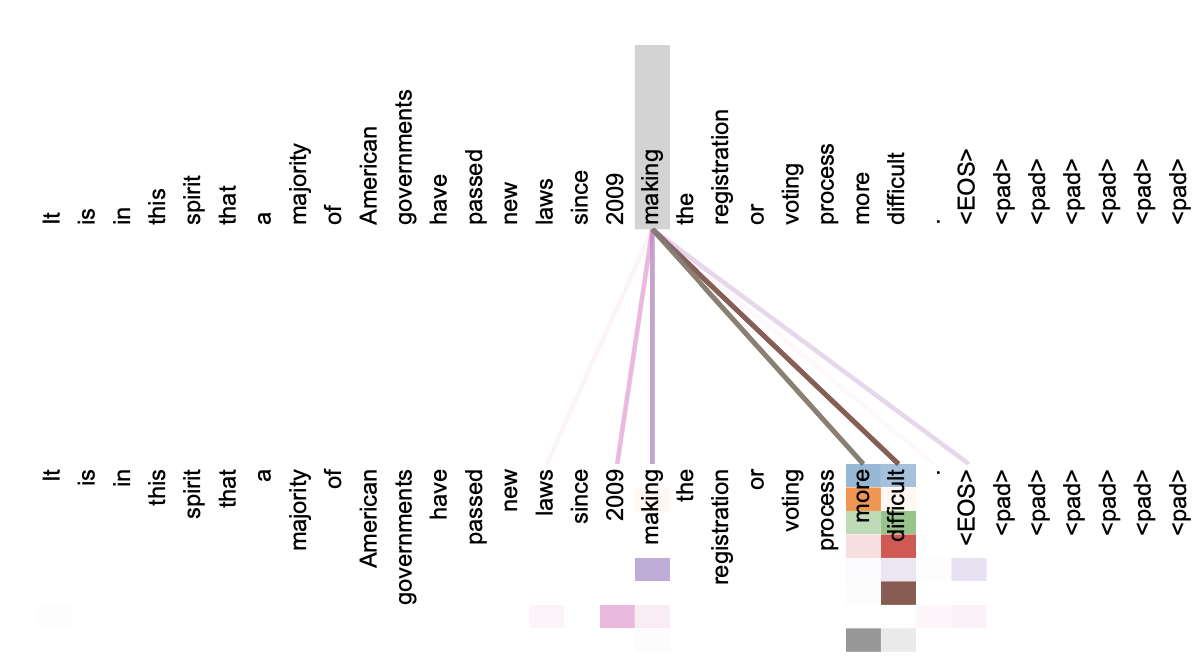
\includegraphics[width=\textwidth]{background_interpretability/vaswani.png}
    \caption{Multi-head attention (with different colors representing different heads) in predicting ``making'', from \citet{vaswani_attention_2017}. Strong weights are placed on ``more difficult'', a phrase directly syntactically linked to ``making''.}
    \label{fig:attention_relevance}
\end{figure}


The weight distribution produced by the softmax function has an implicit interpretation as ``relevance'', strengthening connections between words in a way that draws tempting parallels to latent graph structures in language, like syntactic dependency~\citep{clark_what_2019,voita_analyzing_2019,htut_attention_2019} or constituency~\citep{marecek_balustrades_2019}. This relevance interpretation is seen clearly in Figure~\ref{fig:attention_relevance}, where a close syntactic link in the stereotyped expression ``make \textit{noun} more \textit{adjective}'' is highlighted by the attention distribution. Such methods are convenient but usually limited to attention-based models\footnote{Attention can sometimes be added as a peripheral inactive module for interpretation purposes~\citep{godard_unsupervised_2018}.}.

In settings where we have only one attention distribution when labeling each word, we can ask whether the attention distribution points to, e.g., a parent word or coreferent, as in the \textit{making}-\textit{more} link in Figure~\ref{fig:attention_relevance}. In architectures with \textbf{multi-head} self-attention, multiple attention distributions operate at each layer, so we can no longer point to a single dominant word in a single distribution~\citep{limisiewicz_syntax_2020}. Instead, a common way to measure the syntacticity of the attention distributions is to count the performance of the ``best'' head for a particular relation or instance of the relation~\citep{voita_analyzing_2019,clark_what_2019}. This strategy considers a particular head to be best for a relation like subject-verb, that focuses on a different head in calculating syntacticity when a different relation appears, such as object-verb.

In general, the topmost encoder layers of machine translation (MT) models and the middle layers in Transformer-based LMs like BERT~\citep{Devlin2019BERTPO} and GPT-2~\citep{Radford2019LanguageMA} align with syntactic intuition~\citep{limisiewicz_syntax_2020}.
% \citet{limisiewicz_syntax_2020} point out that MT models follow LM models in the sense that the top of the encoder is also situated in the middle of the encoder-decoder MT architecture.

\paragraph{Is attention interpretable?}

Debate rages over whether attention can be interpreted as word importance in this way~\citep{jain_attention_2019,serrano_is_2019,wiegreffe_attention_2019,vashishth_attention_2019,brunner_validity_2019}, not least because of their limited capabilities on long sequences~\citep{hahn_theoretical_2019,brunner_validity_2019} and the availability of model-agnostic alternatives like saliency~\citep{Bastings2020TheEI}. Regardless of their faithfulness and validity, attention-based analyses of structure are simple to implement and often align with intuition in their results. Even in theory, key-value pairs may mutually amplify each other during training \citep{lu_dynamics_2020}, so we can generally gain some intuition about the internal workings of attention models by observing their weight. Attention-based interpretation methods therefore continue to be in common use today~\citep{belinkov_analysis_2018,rogers_primer_2020}, and observations of attention distributions during training could help extend much of the work in this thesis to modern attentional models.
 
 \subsection{Contextual Decomposition}
 
If we want to consider not just the importance of each word in a sequence, but the causal contribution that entire sets of words make towards a model's output vector, we can use \textbf{Contextual Decomposition} (CD), proposed by \citet{murdoch_beyond_2018}. CD is a way of approximating these influences in an LSTM without adding an attention mechanism or training an additional model (as in DCs).

In the language of CD, we consider the hidden and output vectors produced by an LSTM module to be the sum of \textbf{relevant} and \textbf{irrelevant} parts, the contributions respectively of the \textbf{in-focus} and \textbf{out-of-focus} words in a sequence. For example, we might decompose the hidden layer into contributions of the relevant word set $\beta$ and the irrelevant word set $\bar{\beta}$, producing:

\begin{equation}
    h = h^t_{\beta} + h^t_{\bar{\beta}}
\end{equation}

This is not a trivial decomposition, because the LSTM module applies nonlinearities at each gate, the sigmoid and tanh functions, as shown in Section~\ref{sec:lstm}. CD therefore finds an approximate decomposition of the hidden state by linearizing each gate operation. 

For example, \citet{murdoch_beyond_2018} use a linearized approximation $L_{\sigma}$ for $\sigma$ (and similarly a linearized approximation $L_{\tanh}$ for $\tanh$) such that for arbitrary input $\sum_{j=1}^{N} y_j$: 
\begin{equation}\label{eqn:linear1}
\sigma{\left(\sum_{j=1}^{N} y_j\right)} = \sum_{j=1}^{N} L_{\sigma}(y_j)
\end{equation}

These approximations are then used to split each gate into components contributed by the previous hidden state $h^{t-1}$ and by the current input $x^t$, for example the input gate $i^t$:
\begin{equation} 
\begin{aligned}
i^t &=& \sigma(W_i x^t + V_t h^{t-1} + b_i)\\
&\approx& L_{\sigma}(W_i x^t) + L_{\sigma}(V_t h^{t-1}) + L_{\sigma}(b_i)
\end{aligned}
\end{equation}

The linear form $L_{\sigma}$ is achieved by computing the Shapley value~\citep{shapley_stochastic_1953} of its parameter, defined as the average difference resulting from excluding the parameter, over all possible permutations of the input summants. To apply Formula~\ref{eqn:linear1} to $\sigma{(y_1 + y_2)}$ for a linear approximation of the isolated effect of the summant $y_1$:
\begin{equation}
L_{\sigma}(y_1) = \frac{1}{2} [(\sigma(y_1) - \sigma(0)) + (\sigma(y_2 + y_1) - \sigma(y_1)) ]
\end{equation}

With this function, we can take a hidden state from the previous timestep, decomposed as $h^{t-1} \approx h^{t-1}_{\beta} + h^{t-1}_{\bar{\beta}}$ and add $x^t$ to the appropriate component. For example, if $x^t$ is in focus, we count it in the relevant function inputs when computing the input gate:
\begin{eqnarray*}
i^t &=& \sigma(W_i x^t + V_t h^{t-1} + b_i)\\
&\approx& \sigma(W_i x^t + V_t (h^{t-1}_{\beta} + h^{t-1}_{\bar{\beta}}) + b_i)\\
&\approx& [L_{\sigma}(W_i x^t + V_t h^{t-1}_{\beta}) + L_{\sigma}(b_i)]\\ 
&&+ L_{\sigma}(V_t h^{t-1}_{\bar{\beta}})\\ 
&=& i^t_{\beta} + i^{t}_{\bar{\beta}}
\end{eqnarray*}{}

This provides an expression of the approximate input gate as the sum of relevant and irrelevant components. By ignoring the irrelevant components while computing the module output $h^t$, we produce $h^t_{\beta}$. Thus we linearize and isolate the effect of $\beta$.

In order to isolate $h^t_{\beta}$ from the context, the irrelevant component contains all nonlinear interactions between in-focus and out-of-focus words. We extend CD to analyze these interactions between words in Chapter~\ref{chapter:interdependence}, leading to a new perspective on how an LSTM constructs meaning over the course of training. 

Although CD is particular to the LSTM architecture, the principle behind it is that of the Shapley decomposition, which is general across architectures. Therefore, this generalization of word importance has parallels in other architectures. Shapley values have been used to understand the contribution of entire sets of words over an entire activation vector in many environments~\cite{Lundberg2017AUA,chen_l-shapley_2018,ghorbani_neuron_2020,zhang_inducing_2020}. The existence of such work suggests possible generalizations of any research based on CD to other architectures.


% \todo{Explain Shapley values better}

% \section{Language Interpretation Techniques in This Thesis}

\section{The Perils of Creationism}

For centuries, Europeans agreed that the presence of a cuckoo egg was a great honor to a nesting bird, as it granted an opportunity to exhibit Christian hospitality. The devout bird enthusiastically fed her holy guest, even more so than she would her own (evicted) chicks \citep{davies_cuckoo_2015}. In 1859, Charles Darwin's studies of another occasional brood parasite, finches, called into question any rosy, cooperative view of bird behavior \citep{darwin1964origin}. Without considering the evolution of the cuckoo's role, it would have been difficult to recognize the nesting bird not as a gracious host to the cuckoo chick, but as an unfortunate dupe.

Whether looking at parasitic brooding behavior or at the inner representations of a neural network, if we do not consider how a system develops, it is difficult to distinguish a pleasing story from a useful analysis. In NLP, how can we know if a pattern emerges as informative structure which is used by the model? Apparent syntactic patterns may well be vestigial effects from strategies early in training,\footnote{For one origin story, see the Information Bottleneck Hypothesis, Section \ref{sec:bottleneck}.} or even side effects of training, input structure encodings with no bearing on the final predictions. We consider similarity (Chapter~\ref{chapter:svcca}) and sparsity (Chapter~\ref{chapter:sparsity}) not at one checkpoint, but throughout training. We even illustrate how an LSTM's training strategy makes it well-suited to hierarchical structured data (Chapter~\ref{chapter:interdependence}). These analyses lend a dimension to our understanding that is missing from the "creationist" view of a single checkpoint, manifested without history or evolution.